\documentclass[border=2pt]{standalone}
\usepackage{tikz}
\usetikzlibrary{arrows.meta,chains,%
                    decorations.pathreplacing}
\usetikzlibrary{matrix,positioning,arrows.meta,arrows}
\usetikzlibrary{calc}
\usetikzlibrary{shapes.multipart}
\tikzset{
mymat/.style={
  matrix of nodes,
  nodes in empty cells,
  text height=2.5ex,
  text depth=0.75ex,
  text width=3.25ex,
  align=center,
  column sep=-\pgflinewidth
  },
cartesian/.style={
  align=center, inner sep=1pt, text centered,
  font=\sffamily, circle, black, draw=black, 
  fill=white, text=black, minimum width=0.5em, minimum height=1em
  },
stack/.style={
  rectangle split, rectangle split parts=#1,draw, anchor=center, minimum width=2.5em
  },
three sided/.style={
  draw=none,
  append after command={
      [shorten <= -0.5\pgflinewidth]
      ([shift={(-1.5\pgflinewidth,-0.5\pgflinewidth)}]\tikzlastnode.north east)
  edge([shift={(-1.0\pgflinewidth,+0.5\pgflinewidth)}]\tikzlastnode.south east) 
      ([shift={( 0.5\pgflinewidth,-0.5\pgflinewidth)}]\tikzlastnode.north west)
  edge([shift={( 0.5\pgflinewidth,+0.5\pgflinewidth)}]\tikzlastnode.south west)            
      ([shift={( 0.5\pgflinewidth,+0.5\pgflinewidth)}]\tikzlastnode.south west)
  edge([shift={(-1.0\pgflinewidth,+0.5\pgflinewidth)}]\tikzlastnode.south east)
  },
    every two node part/.style={ rectangle,
                          draw,
                          double,
                          double distance=1mm}
  },
four sided/.style={
        draw=none,
        append after command={
            [shorten <= -0.5\pgflinewidth]
            ([shift={(-1.5\pgflinewidth,-0.5\pgflinewidth)}]\tikzlastnode.north east)
        edge([shift={( 0.5\pgflinewidth,-0.5\pgflinewidth)}]\tikzlastnode.north west) 
            ([shift={( 0.5\pgflinewidth,-0.5\pgflinewidth)}]\tikzlastnode.north west)
        edge([shift={( 0.5\pgflinewidth,+0.5\pgflinewidth)}]\tikzlastnode.south west)            
            ([shift={( 0.5\pgflinewidth,+0.5\pgflinewidth)}]\tikzlastnode.south west)
        edge([shift={(-1.0\pgflinewidth,+0.5\pgflinewidth)}]\tikzlastnode.south east)
            ([shift={(-1.5\pgflinewidth,-0.5\pgflinewidth)}]\tikzlastnode.north east)
        edge([shift={(-1.0\pgflinewidth,+0.5\pgflinewidth)}]\tikzlastnode.south east) 
        }
    }
}
\tikzset{
  rows/.style 2 args={
    sub@rows/.style={row ##1 column #2/.style={nodes={rectangle,draw=black}}},
    sub@rows/.list={#1}
  },
  box/.style 2 args={
    sub@box/.style={rows={#1}{##1}},
    sub@box/.list={#2}
  }
}
\begin{document}

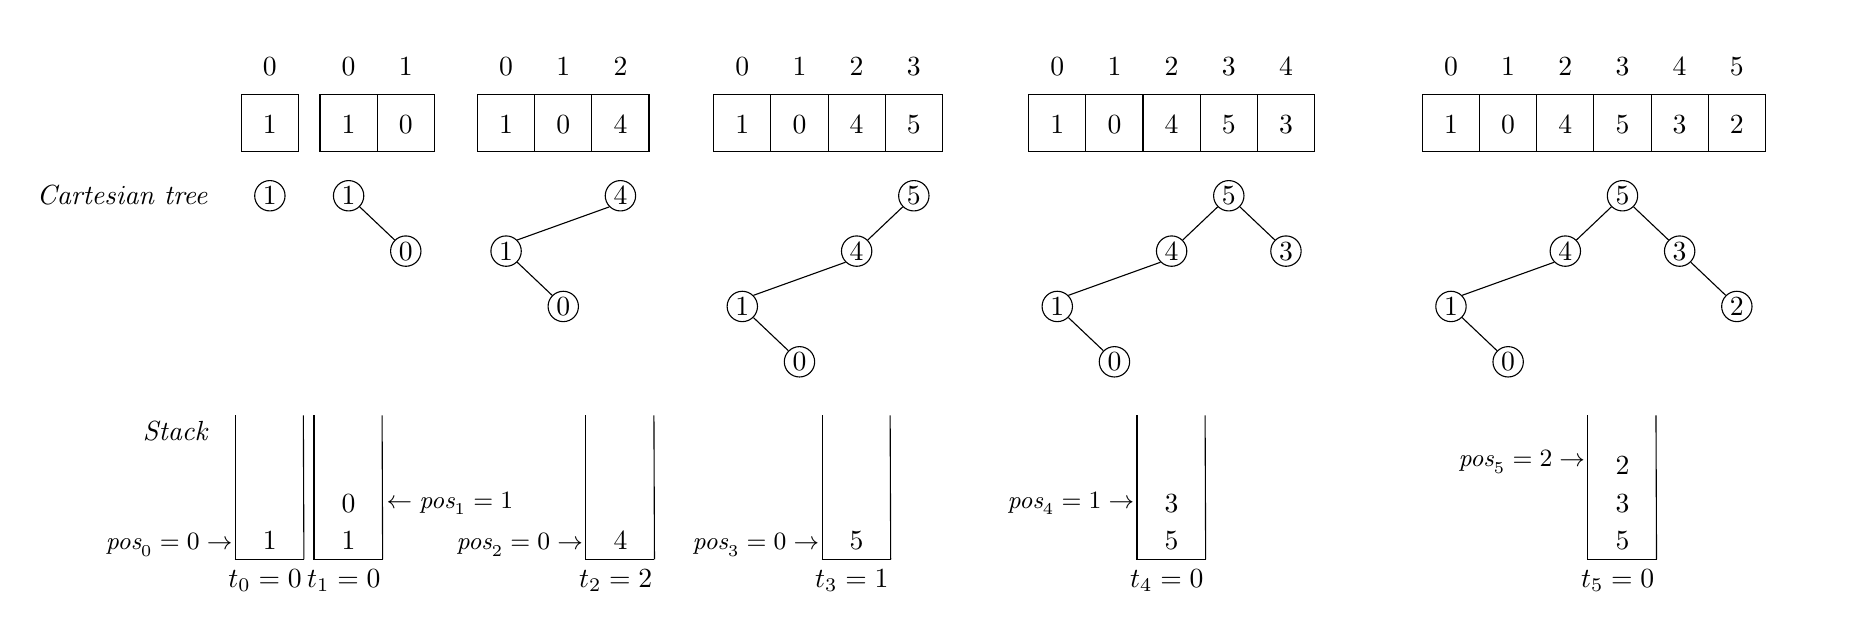
\begin{tikzpicture}[>=latex]
\matrix[mymat,anchor=west,
    box={2}{1}]
at (0,0) 
(mat1)
{ 
  0 & \\
  1 & \\ };
\matrix[mymat,anchor=west,
    box={2}{1, 2}]
at (1,0) 
(mat2)
{ 
  0 & 1 & \\
  1 & 0 & \\ };
\matrix[mymat,anchor=west,
    box={2}{1, 2, 3}]
at (3,0) 
(mat3)
{ 
  0 & 1 & 2 & \\
  1 & 0 & 4 & \\ };
\matrix[mymat,anchor=west,
    box={2}{1, 2, 3, 4}]
at (6,0) 
(mat4)
{ 
  0 & 1 & 2 & 3 & \\
  1 & 0 & 4 & 5 & \\ };
\matrix[mymat,anchor=west,
    box={2}{1, 2, 3, 4, 5}]
at (10,0) 
(mat5)
{ 
  0 & 1 & 2 & 3 & 4 & \\
  1 & 0 & 4 & 5 & 3 & \\ };
\matrix[mymat,anchor=west,
    box={2}{1, 2, 3, 4, 5, 6}]
at (15,0) 
(mat6)
{ 
  0 & 1 & 2 & 3 & 4 & 5 & \\
  1 & 0 & 4 & 5 & 3 & 2 & \\ };

\node[below left=5pt and 5pt of mat1]
{
   $\textit{Cartesian tree}$ \\
};

\node[below left=90pt and 5pt of mat1]
{
   $\textit{Stack}$ \\
};


% step 1

\node[cartesian, below=10pt of mat1-2-1.south](B1-1){$1$};

% step 2

\node[cartesian, below=10pt of mat2-2-1.south](B2-1){$1$};
\node[cartesian, below=30pt of mat2-2-2.south](B2-2){$0$};

\begin{scope}
\draw[](B2-1.south east) -- (B2-2.north west);
\end{scope}

% step 3

\node[cartesian, below=30pt of mat3-2-1.south](B3-1){$1$};
\node[cartesian, below=50pt of mat3-2-2.south](B3-2){$0$};
\node[cartesian, below=10pt of mat3-2-3.south](B3-3){$4$};

\begin{scope}
\draw[](B3-3.south west) -- (B3-1.north east);
\draw[](B3-1.south east) -- (B3-2.north west);
\end{scope}

% step 4

\node[cartesian, below=50pt of mat4-2-1.south](B4-1){$1$};
\node[cartesian, below=70pt of mat4-2-2.south](B4-2){$0$};
\node[cartesian, below=30pt of mat4-2-3.south](B4-3){$4$};
\node[cartesian, below=10pt of mat4-2-4.south](B4-4){$5$};

\begin{scope}
\draw[](B4-4.south west) -- (B4-3.north east);
\draw[](B4-3.south west) -- (B4-1.north east);
\draw[](B4-1.south east) -- (B4-2.north west);
\end{scope}

% step 5

\node[cartesian, below=50pt of mat5-2-1.south](B5-1){$1$};
\node[cartesian, below=70pt of mat5-2-2.south](B5-2){$0$};
\node[cartesian, below=30pt of mat5-2-3.south](B5-3){$4$};
\node[cartesian, below=10pt of mat5-2-4.south](B5-4){$5$};
\node[cartesian, below=30pt of mat5-2-5.south](B5-5){$3$};

\begin{scope}
\draw[](B5-4.south west) -- (B5-3.north east);
\draw[](B5-4.south east) -- (B5-5.north west);
\draw[](B5-3.south west) -- (B5-1.north east);
\draw[](B5-1.south east) -- (B5-2.north west);
\end{scope}

% step 6

\node[cartesian, below=50pt of mat6-2-1.south](B6-1){$1$};
\node[cartesian, below=70pt of mat6-2-2.south](B6-2){$0$};
\node[cartesian, below=30pt of mat6-2-3.south](B6-3){$4$};
\node[cartesian, below=10pt of mat6-2-4.south](B6-4){$5$};
\node[cartesian, below=30pt of mat6-2-5.south](B6-5){$3$};
\node[cartesian, below=50pt of mat6-2-6.south](B6-6){$2$};

\begin{scope}
\draw[](B6-4.south west) -- (B6-3.north east);
\draw[](B6-4.south east) -- (B6-5.north west);
\draw[](B6-5.south east) -- (B6-6.north west);
\draw[](B6-3.south west) -- (B6-1.north east);
\draw[](B6-1.south east) -- (B6-2.north west);
\end{scope}

% stack

\node[stack=4, three sided, below=95pt of mat1-2-1.south](stack1)  {
\nodepart{two}$\phantom{0}$
\nodepart{three}$\phantom{0}$
\nodepart{four}$1$
};

\node[stack=4, three sided, below=95pt of mat2-2-1.south](stack2)  {
\nodepart{two}$\phantom{0}$
\nodepart{three}$0$
\nodepart{four}$1$
};

\node[stack=4, three sided, below=95pt of mat3-2-3.south](stack3)  {
\nodepart{two}$\phantom{0}$
\nodepart{three}$\phantom{0}$
\nodepart{four}$4$
};

\node[stack=4, three sided, below=95pt of mat4-2-3.south](stack4)  {
\nodepart{two}$\phantom{0}$
\nodepart{three}$\phantom{0}$
\nodepart{four}$5$
};

\node[stack=4, three sided, below=95pt of mat5-2-3.south](stack5)  {
\nodepart{two}$\phantom{0}$
\nodepart{three}$3$
\nodepart{four}$5$
};

\node[stack=4, three sided, below=95pt of mat6-2-4.south](stack6)  {
\nodepart{two}$2$
\nodepart{three}$3$
\nodepart{four}$5$
};

% information each operation

\node[below left=0pt and -15pt of stack1.south]
{
   $t_0 = 0$
};

\node[below left=-13pt and 10pt of stack1.south]
{\small
   $\textit{pos}_0 = 0 \rightarrow$
};

\node[below left=0pt and -15pt of stack2.south]
{
   $t_1 = 0$
};

\node[below left=-28pt and -63pt of stack2.south]
{\small
   $\leftarrow \textit{pos}_1 = 1$
};

\node[below left=0pt and -15pt of stack3.south]
{
   $t_2 = 2$
};

\node[below left=-13pt and 10pt of stack3.south]
{\small
   $\textit{pos}_2 = 0 \rightarrow$
};

\node[below left=0pt and -15pt of stack4.south]
{
   $t_3 = 1$
};

\node[below left=-13pt and 10pt of stack4.south]
{\small
   $\textit{pos}_3 = 0 \rightarrow$
};

\node[below left=0pt and -15pt of stack5.south]
{
   $t_4 = 0$
};

\node[below left=-28pt and 10pt of stack5.south]
{\small
   $\textit{pos}_4 = 1 \rightarrow$
};

\node[below left=0pt and -15pt of stack6.south]
{
   $t_5 = 0$
};

\node[below left=-43pt and 10pt of stack6.south]
{\small
   $\textit{pos}_5 = 2 \rightarrow$
};

\end{tikzpicture}

\end{document}